%==================================================================================================
\subsection{\textit{Large Eddy Simulation}} \label{LES}
%==================================================================================================

A simulação de grandes vórtices se baseia na observação de que vórtices formados em pequenas escalas possuem comportamento isotrópico, o que permite uma modelagem dessas escalas, enquanto as grandes escalas podem ser computadas diretamente. Assim, realiza-se uma separação de escalas por meio de um filtro, que irá reescrever as equações de Navier-Stokes em termos de parcelas filtradas (ou de grandes escalas), denotadas para uma propriedade qualquer como $\bar{\phi}$, e uma parcela não filtrada (ou de escalas finas ou flutuações), denotada como $\phi'$ \cite{germano1991dynamic,hughes2000large,moeng2015large}. Para isso, considera-se uma filtragem dada por:

\begin{equation}
    \bar{\phi}=\int_{\Dfil}{g(\BB{y},\yfil)\phi(\yfil,t)d\yfil}\text{,}
\end{equation}

\noindent em que $\Dfil$ é um subconjunto de $\Omega$ que determina a abrangência do filtro, $\yfil$ é um ponto na vizinhança de $\BB{y}$ e $g$ é o filtro, que deve possuir a propriedade de homogeneidade, $g(\BB{y},\yfil)=g(\BB{y}-\yfil)$.

\citeonline{hughes2000large} apresentam ainda uma possibilidade de abrangência de filtro dada por:

\begin{equation}
    \Dfil=\left\{\yfil\in\mathbb{R}^{n_{sd}}|\rho(\BB{y},\yfil)<\Delta/2\right\}\text{,}
\end{equation}

\noindent na qual $\Delta/2$ é o raio de abrangência do filtro centrado em $\BB{y}$ e $\rho$ é a distância Euclidiana de $\yfil$ à $\BB{y}$. A Figura \ref{fig:Filtro} apresenta esquematicamente o filtro considerado, assim como seu domínio de abrangência.

\begin{figure}[h!]
    \centering
    \caption{Desenho esquemático do filtro considerado.}
    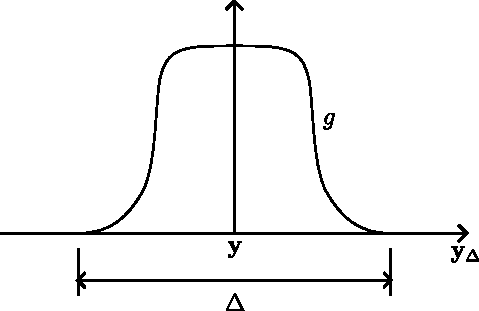
\includegraphics[width=0.5\linewidth]{Figuras/filtro.pdf}
    \\Fonte: \citeonline{hughes2000large} - Adaptado.
    \label{fig:Filtro}
\end{figure}

Dessa maneira, é possível separar os efeitos das grandes escalas e das pequenas escalas, o que pode ser observado esquematicamente na Figura \ref{fig:EfeitoFiltragem}, a qual apresenta o efeito da filtragem sobre um campo de velocidades $\BB{u}$.

\begin{figure}[h!]
    \centering
    \caption{Efeito da filtragem sobre um campo de velocidades $\BB{u}$.}
    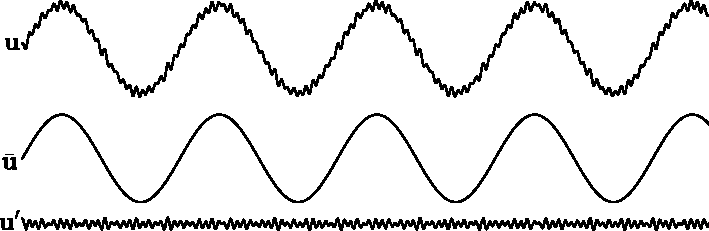
\includegraphics[width=.75\linewidth]{Figuras/efeito_filtragem.pdf}
    \\Fonte: \citeonline{hughes2000large} - Adaptado.
    \label{fig:EfeitoFiltragem}
\end{figure}

Assim, em uma descrição Euleriana, pode-se obter as equações de Navier-Stokes filtradas:

\begin{equation}
    \left\{
    \begin{array}{ll}
        \rho\bigpar{\dot{\bar{u}}_i+(\overline{u_iu_j})_{,j}-\bar{f}_i}-\bar{\sigma}_{ji,j}=0 & \text{ em }\Omega\text{,} \\
        \bar{u}_{i,i}=0                                                                       & \text{ em }\Omega\text{.}
    \end{array}
    \right.
\end{equation}

Pode-se perceber que o termo convectivo impede a completa separação dos termos $\BBB{u}$ e $\BB{u}'$ devido à sua natureza altamente não-linear. Por conta disso a parcela não filtrada não pode ser ignorada nesse problema, sendo necessário realizar algumas manipulações algébricas. Logo, sabendo-se que $\BB{u}=\BBB{u}+\BB{u}'$, pode-se reescrever a equação da conservação de movimento como:

\begin{equation}
    \rho\bigpar{\dot{\bar{u}}_i+(\overline{(\bar{u}_i+u'_i)(\bar{u}_j+u'_j)})_{,j}-\bar{f}_i}-\bar{\sigma}_{ji,j}=0
\end{equation}

Nesse sentido, surgirão termos cruzados entre $\BBB{u}$ e $\BB{u}'$, o que serão condensados em um tensor de subescala (\textit{Subgrid-Scale} - SGS) $\BB{T}$ dado por \cite{piomelli1999large,hughes2000large}:

\begin{equation}
    T_{ij}=\bar{u}_i\bar{u}_j-\overline{u_iu_j}=-\bigpar{L_{ij}+C_{ij}+R_{ij}}\text{,}
\end{equation}

\noindent no qual $L_{ij}=\overline{\bar{u}_i\bar{u}_j}-\bar{u}_i\bar{u}_j$ é o tensor de Leonard, que representa as interações entre as grandes escalas, podendo ser determinado explicitamente utilizado para análise de erros, $C_{ij}=\overline{\bar{u}_iu'_j}+\overline{u'_i\bar{u}_j}$ é o tensor de termos cruzados, representando a interação entre as grandes e pequenas escalas e $R_{ij}=\overline{u'_iu'_j}$ é o tensor de tensões SGS de Reynolds, que rerepsenta a interação entre as pequenas escalas \cite{piomelli1999large}. Assim pode-se escrever que:

\begin{equation}
    \rho\bigpar{\dot{\bar{u}}_j+(\bar{u}_i\bar{u}_j)_{,i}-T_{ij,i}-\bar{f}_j}-\sigma_{ij,i}=0\text{.}
\end{equation}

Aplicando a incompressibilidade e substituindo-se $\sigma_{ij}$ pelo modelo constitutivo \ref{eq:ModConst}, tem-se que:

\begin{equation}
    \rho\bigpar{\dot{\bar{u}}_i+\bar{u}_j\bar{u}_{i,j}-T_{ji,j}-\bar{f}_i}-\mu(\bar{u}_{i,j}+\bar{u}_{j,i})_{,j}+p_{,i}=0\text{,}\label{eq:ConMasLES}
\end{equation}

\noindent Assim, dividindo-se a Equação \ref{eq:ConMasLES} por $\rho$ e fazendo algumas manipulações tem-se que:

\begin{equation}
    \dot{\bar{u}}_i+\bar{u}_j\bar{u}_{i,j}+\frac{p_{,i}}{\rho}=\nu\bar{u}_{i,jj}+T_{ji,j}+\bar{f}_i\text{,}
\end{equation}

\noindent em que $\nu$ é a viscosidade cinemática, dada por $\nu=\mu/\rho$.

Portanto, o problema se ser resolvido será:

\begin{equation}
    \left\{
    \begin{array}{ll}
        \dot{\bar{u}}_i+\bar{u}_j\bar{u}_{i,j}+\frac{p_{,i}}{\rho}=\nu\bar{u}_{i,jj}+T_{ji,j}+\bar{f}_i & \text{ em }\Omega\text{,} \\
        \bar{u}_{i,i}=0                                                                                 & \text{ em }\Omega\text{,}
    \end{array}
    \right.
\end{equation}

\noindent o que revela a necessidade de se determinar um tensor $\BB{T}$, em especial o seu tensor desviador:

\begin{equation}
    \dev{T_{ij}}=T_{ij}-\frac{1}{3}T_{kk}\delta_{ij}\text{,}
\end{equation}

\noindent que descreva adequadamente as interações entre diferentes escalas. Isso pode se tornar problemático uma vez que não se possui solução para as pequenas escalas. Dessa forma, considera-se um modelo capaz de fazer essa descrição, sendo observado, por exemplo, o modelo de viscosidade de vórtice de Smagorinsky, desenvolvido por \citeonline{smagorinsky1963general}. Nesse cenário faz-se que:

\begin{equation}
    \bigpar{T_S}_{ij}=2\nu_T\deffilij{ij}\text{,}
\end{equation}

\noindent sendo $\nu_T$ a viscosidade de vórtice SGS, dada por \cite{germano1991dynamic,piomelli1999large,hughes2000large,bailly2015turbulence,katopodes2019free}:

\begin{equation}
    \nu_T=(C_S\Delta)^2\norm{\deffil}\text{,}
\end{equation}

\noindent em que $C_S$ é a constante de Smagorinsky e $\norm{\deffil}$ é a magnitude do tensor de taxa de deformação em grandes escalas, dada por:

\begin{equation}
    \norm{\deffil}=(2\deffilij{ij}\deffilij{ij})^{1/2}\text{.}
\end{equation}

Note que o tensor $\BB{T}_S$ é um tensor desviador, ou seja, $\BB{T}_S=\dev{\BB{T}_S}$.

\citeonline{germano1991dynamic,hughes2000large} ainda fazem algumas constatações sobre o modelo de Smagorinsky, os quais destacam-se o fato de $\BB{T}_S$ não possuir um comportamento assintótico próximo às paredes, o que se esperaria de $\BB{T}$, os valores de $C_S$ na presença de cisalhamento médio causaram amortecimentos excessivos e o tensor $\BB{T}_S$ impede a energia de fluir entre diferentes escalas, podendo ser significante em alguns casos.

Como tentativa de se resolver esses problemas, \citeonline{germano1991dynamic} propuseram assumir $C_S$ como uma função $C_S=C_S(\BB{y},t)$, permitindo, assim, que esse parâmetro se adapte para melhor modelar as pequenas escalas.

Assim, define-se inicialmente a amplitude espectral da energia cinética $E(k)$, dada sobre uma superfície de esferas parametrizadas de raio $k$, dada por \cite{hughes2000large}:

\begin{equation}
    E(k)=\alpha\varepsilon^{2/3}k^{-5/3}\text{,}\label{eq:Ek1}
\end{equation}

\noindent em que $\alpha$ é a constante de Kolmogoroff, $\varepsilon$ é a dissipação turbulenta. A Figura \ref{fig:EnergiaEspectral} apresenta graficamente o comportamento da energia espectral:

\begin{figure}[h!]
    \centering
    \caption{Energia espectral de Kolgomorov.}
    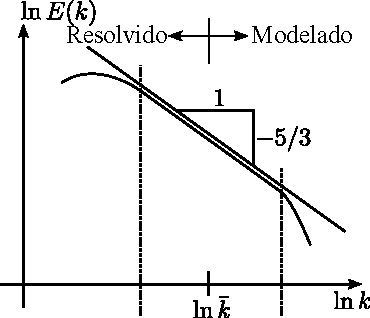
\includegraphics[width=0.4\linewidth]{Figuras/EnergiaEspectral.pdf}
    \\Fonte: \cite{hughes2000large} - Adaptado.
    \label{fig:EnergiaEspectral}
\end{figure}

Logo pode-se determinar o valor de $\norm{\deffil}$ como:

\begin{equation}
    \frac{1}{2}\norm{\deffil}=\int_0^{\bar{k}}{k^2E(k)dk}\text{,}\label{eq:ndeffil1}
\end{equation}

\noindent no qual $\bar{k}$ é o limite de resolução.

Substituindo \ref{eq:Ek1} em \ref{eq:ndeffil1}, resolvendo a integral e fazendo algumas manipulações algébricas, tem-se que:

\begin{equation}
    \norm{\deffil}^3=\bigpar{\frac{3\alpha}{2}}^{3/2}\bar{k}^2\varepsilon\text{.}
\end{equation}

Com isso, considerando também que a dissipação de energia cinética é igual àquela produzida, realiza-se o balanço da energia, obtendo-se:

\begin{equation}
    \varepsilon=({T}_S)_{ij}\deffilij{ij}\text{,}
\end{equation}

\noindent que, após seu desenvolvimento, tem-se uma expressão que relaciona os valores de $C_S$, $\Delta$ e $\nu_T$ com $\bar{k}$:

\begin{equation}
    C_S\Delta=\bigpar{\frac{2}{3\alpha}}^{3/4}\bar{k}^{-1}\text{ e}
\end{equation}

\begin{equation}
    \nu_T=\bigpar{\frac{2}{3\alpha}}\varepsilon^{1/3}\bar{k}^{-4/3}\text{.}
\end{equation}

Segundo \citeonline{bailly2015turbulence} o valor de $\bar{k}$ pode ser estimado como:

\begin{equation}
    \bar{k}=\frac{\pi}{\Delta}\text{,}
\end{equation}

\noindent o que leva à seguinte expressão para a constante de Smagorinsky:

\begin{equation}
    C_S=\frac{1}{\pi}\bigpar{\frac{2}{3\alpha}}^{3/4}\text{.}
\end{equation}

Com isso, um possível valor para a constante Kolmogoroff é $\alpha=1,4$, o que resulta em $C_S\approx0,18$. No entanto valores de $C_S$ próximos à 0,10 conduzem a solução à resultados mais realistas \cite{hughes2000large,bailly2015turbulence,katopodes2019free}.

%==================================================================================================
\subsubsection{Procedimento computacional} \label{LES-PC}
%==================================================================================================

Para a obtenção dos resultados, parte-se para a formulação variacional, em que se utiliza funções testes $\BB{w}$ e $q$, associadas às equações de conservação do momento e da continuidade, respectivamente. Assim, se tem a forma fraca do problema, dada por:

\begin{equation}
    \begin{split}
        &\intDom{w_i\rho\bigpar{\dot{\ub}_i+\uub{j}\ub_{i,j}-\bar{f}_i}}+\intDom{\rho w_{i,j}T_{ij}}+\intDom{w_{i,j}\sigma_{ji}(\BB{\ub},\pb)}+\\
        &\intDom{q\ub_{i,i}}-\intNeumann{\rho w_iT_{ij}n_j}-\intNeumann{w_i\bar{h}_i}=0\text{.}
    \end{split}
\end{equation}

Substituindo o modelo constitutivo e o modelo de viscosidade de Smagorinsky tem-se que:

\begin{equation}
    \begin{split}
        &\intDom{w_i\rho\bigpar{\dot{\ub}_i+\uub{j}\ub_{i,j}-\bar{f}_i}}+\intDom{w_{i,j}(\mu+\rho\nu_T)(\uSim{\ub}{i}{j})}-\\
        &\intDom{w_{i,i}\pb}+\intDom{q\ub_{i,i}}-\intNeumann{w_i\bar{h}_i}=0\text{.}
    \end{split}
\end{equation}

No intuito de se obter uma solução estável, será considerado o elemento de Taylor-Hood P2P1 (aproximação quadrática para o campo de velocidades e linear para o campo de pressões) na formulação. Assim denomina-se $M$ as funções de forma para aproximação quadrática e $N$ para funções de forma lineares. Com isso, faz-se a aproximação das funções testes por meio das funções de forma, tendo como resultado os seguintes vetores de resíduo associados às equações de conservação de momento e da continuidade:

\begin{subequations}
    \begin{equation}
        \begin{split}
            \bigpar{N_M}_i^a=&\intDom{M_a\rho\bigpar{\dot{\ub}_i+\uub{j}\ub_{i,j}-\bar{f}_i}}+\\
            &\intDom{M_{a,j}(\mu+\rho\nu_T)(\uSim{\ub}{i}{j})}-\intDom{M_{a,i}\pb}-\intNeumann{N_a\bar{h}_i}\text{ e}
        \end{split}
    \end{equation}
    \begin{equation}
        \bigpar{N_C}^a=\intDom{N_a\ub_{i,i}}\text{.}
    \end{equation}
    \label{eq:VetoresResiduo-LES}
\end{subequations}

Dessa forma procura-se determinar valores de $\ub$ e $\pb$ que anulem $N_M$ e $N_C$. Para esse fim utiliza-se o método de Newton-Raphson, em que os parâmetros a serem determinados são as acelerações e pressões nodais, sendo o integrador utilizado o $\alpha$-generalizado, apresentado na seção \ref{IT-VMS}. Desse modo tem-se os seguintes sub-blocos que compõem a matriz tangente:

\begin{subequations}
    \begin{equation}
        \begin{split}
            \der{(N_M)_i^a}{\dot{U}_j^b}=&\alpha_m\intDom{\rho M_aM_b}\dij+\beta_f\intDom{\rho M_aM_b\ub_{i,j}}+\\
            &\beta_f\intDom{\rho M_aM_{b,k}\uub{k}}\dij+\beta_f\intDom{(\mu+\rho\nu_T)M_{a,k}M_{d,k}}\dij+\\
            &\beta_f\intDom{(\mu+\rho\nu_T)M_{a,j}M_{b,i}}\text{,}
        \end{split}
    \end{equation}
    \begin{equation}
        \der{(N_M)_i^a}{P^b}=-\intDom{M_{a,i}N_b}\text{,}
    \end{equation}
    \begin{equation}
        \der{(N_C)^a}{\dot{U}_j^b}=\beta_f\intDom{N_aM_{b,j}}\text{ e}
    \end{equation}
    \begin{equation}
        \der{(N_C)^a}{P^b}=0\text{.}
    \end{equation}
    \label{eq:MatrizTangente-LES}
\end{subequations}

\noindent em que $\beta_f=\alpha_f\gamma\Delta t$.

Observa-se que o sub-bloco $\partial{\NC}/\partial\BB{P}$ está presente na diagonal principal do problema, possuindo valor nulo. Isso pode ser interpretado como a consideração das pressões como multiplicadores de Lagrange nessa formulação.

Para obtenção da solução aproximada, utiliza-se um procedimento similar ao apresentado no algoritmo \ref{alg:MEF-VMS}, onde o comando \ref{alg:estabilizador} é alterado para computar o valor da viscosidade de vórtice, assim como os valores das componentes da matriz tangente e dos vetores de resíduo são alterados para se adequarem ao presente modelo.